%!TEX root = ../template.tex
%%%%%%%%%%%%%%%%%%%%%%%%%%%%%%%%%%%%%%%%%%%%%%%%%%%%%%%%%%%%%%%%%%%%
%% chapter4.tex
%% NOVA thesis document file
%%
%% Chapter with lots of dummy text
%%%%%%%%%%%%%%%%%%%%%%%%%%%%%%%%%%%%%%%%%%%%%%%%%%%%%%%%%%%%%%%%%%%%
\chapter{Planning} \label{cha:planning}

In this Chapter we begin by defining the system model and the intuition for the proposed solution followed by defining a set of metrics to evaluate it. Finally, in the last section we present the work plan for the remaining of the thesis. 

As previously mentioned, the challenge we propose to address is to create a large-scale decentralized management and monitoring infrastructure tailored for heterogenous edge devices, which in turn may be used to track the state of applications (for load balancing), discover nearby devices to offload tasks, or find a set of devices to deploy a new application in a strategic location, enabling in the future the autonomic management of edge-enabled applications.

\section{System Model}

As defined in Section~\ref{sec:edge_computing}, the edge environment is composed by devices classified in levels ranging from [0-7]. From this classification, we outline two major categories:  

\textbf{Stable devices} consist of devices ranging from levels [0-5] in the taxonomy. We consider devices in these levels ``stable'' because they are usually connected across a wired medium (except in the case of laptops) which makes their connections more stable, and have enough computational capacity to perform monitoring and management tasks.

\textbf{Unstable devices} are comprised by devices in levels 6 and 7. In the case of mobile devices (level 6), we consider them unstable due to their low computational power and the fact that their physical location may change rapidly, which may lead to topology mismatch. Furthermore, both devices in levels 6 and 7 are connected across a wireless medium which raises a large number of concerns which are outside the scope of this work.

Following, we have the applications, in the context of this thesis, we will only consider the management of \textbf{edge-enabled applications} running on containers. We consider these as applications which are decomposable into independent components, these application components may be hosted in a single container, and function as a \textit{monolithic} application, or alternatively have components hosted by devices scattered throughout the system. 

Consequently, we define a set of operations which are critical for this type of applications: \textit{offloading} and \textit{migrating}. Offloading consists in delegating the task of hosting an application subcomponent to another device, whereas migrating means transferring a component (or multiple components) of the application to another device in the system. T

These two operations enable load-balancing the application through offloading tasks, enable scaling up or down depending on the computational capabilities of the device, and allow applications to improve their latency by migrating or offloading application components to devices near the end-users. 

%%%%%%%%%%%%%%%%%%%%%%%%%%%%%%%%%%%%%%%%%%%%%%%%%%%%%%%%%%%%%%%%%%
\section{Proposed Solution}
\label{cha:proposed_sol}

As previously mentioned, the challenge we propose to address is to create a large-scale decentralized management and monitoring infrastructure tailored for heterogenous edge devices, which in turn may be used to track the status of applications, discover nearby devices to offload tasks, or find devices to deploy a set of services given certain constraints. 

\begin{figure}
    \centering
    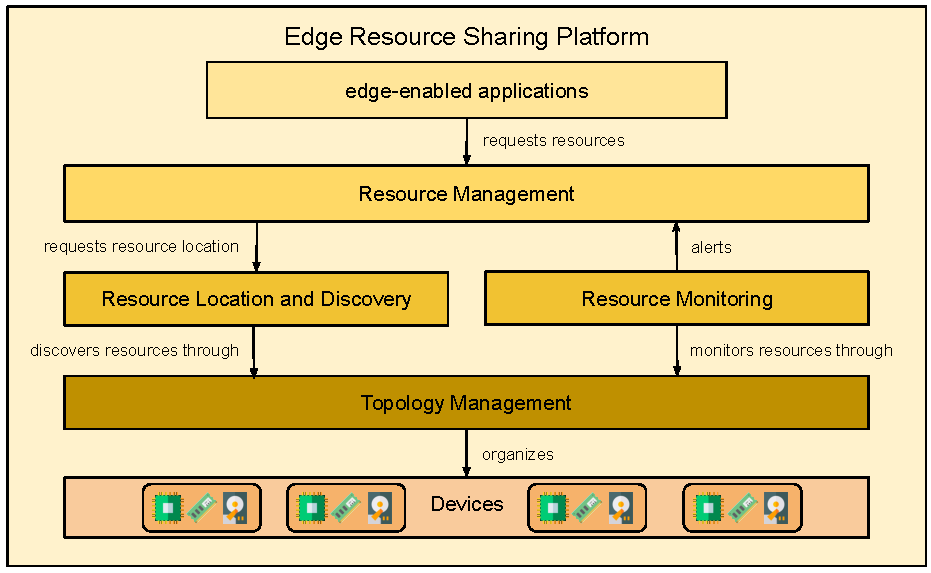
\includegraphics[width=0.9\linewidth]{Figures/proposed_architecture_detailed.pdf}
    \caption{High-level architecture of the proposed resource sharing platform}
    \label{fig:proposed_architecture_detailed}
\end{figure}

In the Figure \ref{fig:proposed_architecture_detailed}, we find the proposed architecture of the solution we intend to design, which is composed of four co-dependent mechanisms exercised by every participant of the system.

At the bottom we have topology management, whose responsibilities consist of: (1) ensuring that devices belonging to the overlay remain connected at all times; (2) materializing a hierarchical topology inspired on the capabilities of devices composing the system; (3) assure that devices have at least one non-faulty device connected to it. This mechanism enables the correct behavior of the remaining components.

Following, we have resource monitoring, the objectives of this mechanism consist in collecting metrics regarding the tasks running and the free resources in nearby devices, in addition to detecting if an application hosted on certain device is not performing according to the established performance criteria, and emit alerts which in turn may trigger either an application migration, or the offload of a certain task.

Next, we have resource location and discovery, this mechanism offers search strategies such that nodes can cooperatively find available resources in the system so that a node hosting a certain application has available targets to offload tasks to.

Finally, we have resource management, which consists in a mechanism which handles the alerts emitted, and performs migration or offloading decisions based on the information reported by the alerts.

\section{Evaluation}  

In order to evaluate our work, we will employ a real-world scenario composed by devices ranging across the different levels of capacity and availability. The devices composing the test scenario consist of: devices in Cloud Environments (e.g. AWS or azure), devices in the Grid5000 cluster and around 20 Raspberry Pis.

In order to evaluate the implemented solution, and the advantages and disadvantages of the decentralized hierarchical model, we intend to develop two variants of monitoring systems. The first and most popular approach consists of a centralized controller tracking the state of devices and applications running on them. The second approach consists of a flat decentralized model, in this model, peers are not organized into a hierarchy and simply exchange monitoring information with other peers in the system. These simple solutions will serve as a baseline for our own solution.

We define a set of system and applicational-related metrics in order to compare the aforementioned implementations. The \textbf{system metrics} consist of the usage of system resources such as cpu, memory and bandwidth in each node of the system, followed by the number of required messages to maintain the overlay.

\textbf{Application metrics} consist in metrics related to the monitoring infrastructure running atop the overlay. The first metric to consider is cost, which consists in the relation between the number of messages sent and the value of the information. Following, we have information freshness, which consists in the timeliness of the information each node has of the system. Finally, we have information precision, which represents the difference between the obtained monitoring data and the real status of the device / applications running on it.  

\section{Scheduling}

In this section we outline the identified tasks and present the work plan in order to accomplish the established objectives. We identify four main tasks: first task is to devise, implement and validate the hierarchical overlay network. Following, the second task consists of implementing and validating the decentralized monitoring system. The third task is to perform the experimental evaluation of the system, and finally, the final task consists in writing the thesis document.

\begin{enumerate}
    \item Topology management mechanism
    \begin{enumerate}
        \item Implement
        \item Validate
        \item Evaluate
    \end{enumerate}

    \item Resource monitoring mechanism
    \begin{enumerate}
        \item Implement
        \item Validate
        \item Evaluate
    \end{enumerate}
    
\end{enumerate}








